\documentclass[conference]{IEEEtran}

\usepackage{cite}
\usepackage{amsmath,amssymb}
\usepackage{graphicx}
\usepackage{booktabs}
\usepackage{multirow}
\usepackage{xcolor}
\usepackage{url}
\usepackage{tikz}
\usepackage{algorithm}
\usepackage{algorithmic}
\usepackage{array}

\usetikzlibrary{arrows.meta,positioning,shapes.geometric,shapes.misc,fit}

\title{TIM-MARS: A Lightweight Selected-Target Memory Layer for Robust Vision-Based UAV Person Following}

\author{
\IEEEauthorblockN{Francisco Tavares}
\IEEEauthorblockA{
Instituto Superior Técnico, Universidade de Lisboa\\
Lisbon, Portugal\\
Email: francisco.carreira.tavares@gmail.com
}
}

\begin{document}

\maketitle

\begin{abstract}
Reliable person following with micro aerial robots requires more than detecting and tracking people in each frame. When the selected person is occluded, crosses another person, or re-enters the scene, a tracker may continue producing plausible outputs while following the wrong identity. This failure is particularly important for control, where following the wrong person is less safe than temporarily declaring the target lost. This paper presents TIM-MARS, a lightweight selected-target memory layer that operates above a multi-object tracker and uses geometry, tracker state, and MARS appearance embeddings to stabilise the selected target. TIM-MARS publishes a control-facing target state and is evaluated using a selected-target correctness metric that separates correct, wrong, and lost output duration. On a hard re-entry sequence, ByteTrack combined with TIM-MARS improves the correct-target ratio from 68.7\% to 96.9\%, while reducing the wrong-target ratio from 11.5\% to 1.5\%. In a post-detection replay benchmark, ByteTrack + TIM-MARS increases replay-level CPU share from 6\% to 10\% relative to raw ByteTrack, while wall time and peak memory remain nearly unchanged. The results show that, on this stress sequence, selected-target memory can substantially improve control-oriented target robustness when the base tracker has recoverable identity instability.
\end{abstract}


\begin{IEEEkeywords}
UAV perception, target tracking, person following, multi-object tracking, re-identification, edge AI, selected-target memory.
\end{IEEEkeywords}

\section{Introduction}

Vision-based person following is a core capability for micro aerial robots operating in human-centred environments. A typical perception stack detects people, tracks them over time, and forwards a selected target to a downstream controller. However, reliable control requires more than maintaining generic multi-object tracks. The system must preserve the identity of one selected person, especially after occlusion, crossing events, and target re-entry.

This distinction matters because a tracker may produce visually plausible outputs while assigning the selected target to the wrong person. For a following UAV, this is a safety-relevant failure. A lost target can be handled by slowing down, hovering, or stopping target-following behaviour. A wrong target can instead command the robot toward the wrong person. Therefore, this work adopts the control-oriented rule that wrong target is worse than lost target.

This paper presents TIM-MARS, a selected-target memory layer for robust UAV person following. TIM-MARS operates above an existing detector and multi-object tracker. It does not attempt to replace the tracker. Instead, it filters the raw selected-target output using temporal memory, geometric consistency, and MARS re-identification appearance evidence. The result is a control-facing target state that can remain locked, become uncertain, be declared lost, or be reacquired.

The main contributions are:

\begin{itemize}
    \item a selected-target memory formulation focused on control safety rather than generic tracking accuracy;
    \item a lightweight TIM-MARS layer combining tracker state, geometry, and MARS appearance embeddings;
    \item a selected-target correctness evaluation that separates correct, wrong, and lost output duration;
    \item an experimental comparison across ByteTrack, OCSORT, and DeepSORT-MARS on a hard re-entry sequence.
\end{itemize}

The results show that TIM-MARS is most useful when the base tracker has recoverable identity instability. In the evaluated hard re-entry sequence, ByteTrack with TIM-MARS achieves the strongest result, reducing wrong-target output while increasing correct-target duration.

\section{Related Work}

\subsection{Vision-Based UAV Person Following}

Vision-based UAV person following commonly relies on object detection, tracking, and visual servoing or target-relative control. In constrained cases, a detector alone can provide a target location for control. In multi-person scenes, however, the system must also maintain the identity of the selected person. This makes the problem different from generic person detection, because the selected identity must remain stable under occlusion, crossing, and re-entry.

\subsection{Multi-Object Tracking}

Multi-object tracking methods associate detections over time and produce track identities. SORT provides a lightweight online baseline based on Kalman filtering and frame-to-frame association~\cite{bewley2016sort}. DeepSORT extends this idea with an appearance association metric~\cite{wojke2017deepsort}. ByteTrack improves association by using both high-confidence and low-confidence detections~\cite{zhang2022bytetrack}, while OCSORT improves robustness by rethinking the observation and motion update strategy~\cite{cao2023ocsort}. These trackers are usually evaluated with generic tracking metrics. For target-following control, however, the relevant question is narrower: whether the selected person remains the correct control target.

\subsection{Appearance-Based Re-Identification}

Appearance-based re-identification methods use visual descriptors to compare identities across frames. MARS provides a large-scale video benchmark for person re-identification and motivates compact appearance embeddings for identity comparison over time~\cite{zheng2016mars}. In this work, appearance is used as supporting evidence inside a selected-target memory layer rather than as a standalone tracking method.

\subsection{Control-Oriented Target Robustness}

For closed-loop UAV following, identity errors have different consequences from temporary target loss. A lost target can trigger conservative behaviour, while a wrong target may lead to unsafe following. This motivates evaluating selected-target tracking with separate correct, wrong, and lost durations instead of relying only on generic tracking accuracy or output availability.

\section{System Overview}

The perception stack is organised as a detector-tracker-memory-control pipeline. TIM-MARS is inserted above the base tracker and below the controller. It does not replace the tracker; it converts raw selected-track output into a control-facing selected-target state.

\begin{figure*}[t]
\centering
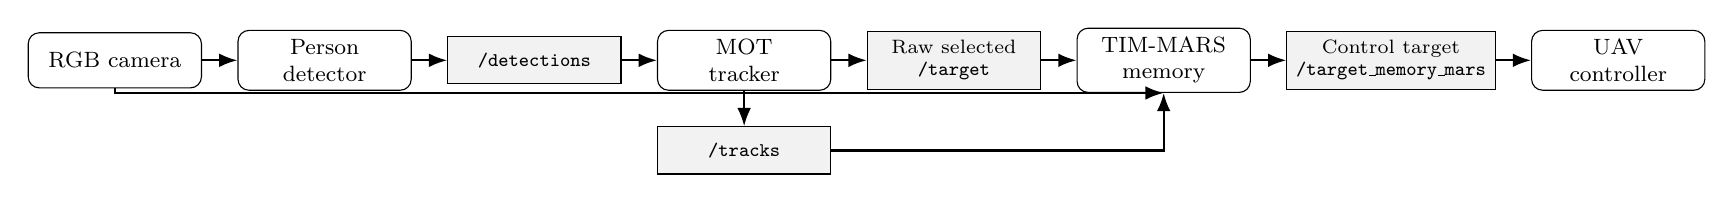
\begin{tikzpicture}[
    node distance=4.5mm,
    block/.style={draw, rounded corners, align=center, minimum width=22mm, minimum height=7mm, font=\footnotesize},
    topic/.style={draw, align=center, minimum width=22mm, minimum height=6mm, font=\scriptsize, fill=gray!10},
    arrow/.style={-Latex, thick}
]
\node[block] (cam) {RGB camera};
\node[block, right=of cam] (det) {Person\\detector};
\node[topic, right=of det] (detections) {\texttt{/detections}};
\node[block, right=of detections] (tracker) {MOT\\tracker};
\node[topic, below=of tracker] (tracks) {\texttt{/tracks}};
\node[topic, right=of tracker] (rawtarget) {Raw selected\\\texttt{/target}};
\node[block, right=of rawtarget] (tim) {TIM-MARS\\memory};
\node[topic, right=of tim] (memtarget) {Control target\\\texttt{/target\_memory\_mars}};
\node[block, right=of memtarget] (ctrl) {UAV\\controller};

\draw[arrow] (cam) -- (det);
\draw[arrow] (det) -- (detections);
\draw[arrow] (detections) -- (tracker);
\draw[arrow] (tracker) -- (rawtarget);
\draw[arrow] (tracker) -- (tracks);
\draw[arrow] (tracks.east) -| (tim.south);
\draw[arrow] (rawtarget) -- (tim);
\draw[arrow] (cam.south) |- (tim.south);
\draw[arrow] (tim) -- (memtarget);
\draw[arrow] (memtarget) -- (ctrl);
\end{tikzpicture}
\caption{TIM-MARS is a selected-target memory layer above the tracker. It filters the raw selected target into a control-facing target state.}
\label{fig:pipeline}
\end{figure*}

The relevant ROS~2 topics are summarised in Table~\ref{tab:topics}.

\begin{table}[t]
\centering
\caption{Main runtime topics used by TIM-MARS.}
\label{tab:topics}
\begin{tabular}{ll}
\toprule
Topic & Role \\
\midrule
\texttt{/detections} & detector output \\
\texttt{/tracks} & base tracker candidates \\
\texttt{/target} & raw selected target \\
\texttt{/target\_memory\_mars} & memory-filtered selected target \\
\texttt{/target\_memory\_mars/status} & diagnostic memory state \\
\bottomrule
\end{tabular}
\end{table}

This structure makes the tracker interchangeable. The same selected-target memory layer can be evaluated with ByteTrack, OCSORT, or DeepSORT-MARS.

\section{TIM-MARS Formulation}

TIM-MARS is implemented as a selected-target memory layer above a tracker. At frame $t$, the tracker provides a candidate set
\begin{equation}
\mathcal{C}_t = \{c_t^1,\ldots,c_t^N\},
\end{equation}
where each candidate is represented as
\begin{equation}
c_t^i = (b_t^i, q_t^i, id_t^i, e_t^i).
\end{equation}
Here, $b_t^i$ is the bounding box, $q_t^i$ is the tracker confidence, $id_t^i$ is the tracker identity, and $e_t^i$ is the MARS appearance descriptor when available.

The memory state is
\begin{equation}
m_t = (b_t^\star, id_t^\star, e_t^\star, s_t, h_t),
\end{equation}
where $b_t^\star$ is the remembered selected-target box, $id_t^\star$ is the remembered tracker identity, $e_t^\star$ is the appearance memory, $s_t$ is the finite memory state, and $h_t$ stores hysteresis counters.

\subsection{Base Candidate Score}

Candidates below a minimum tracker confidence are discarded:
\begin{equation}
\mathcal{C}_t' =
\{c_t^i \in \mathcal{C}_t \mid q_t^i \geq \tau_q\}.
\end{equation}

For each remaining candidate, TIM-MARS computes five terms:
\begin{align}
I_i &= \mathrm{IoU}(b_t^i,b_{t-1}^\star),\\
D_i &= \exp\left[-\frac{1}{2}\left(\frac{d(b_t^i,b_{t-1}^\star)}{\sigma_d}\right)^2\right],\\
Z_i &= \exp\left[-\frac{|\log(A(b_t^i)/A(b_{t-1}^\star))|}{\sigma_z}\right],\\
Q_i &= \mathrm{clip}(q_t^i,0,1),\\
B_i &=
\begin{cases}
1, & id_t^i = id_{t-1}^\star,\\
0, & \mathrm{otherwise}.
\end{cases}
\end{align}

The base score is
\begin{equation}
S_i^{0}
=
w_I I_i
+
w_D D_i
+
w_Z Z_i
+
w_Q Q_i
+
w_B B_i.
\end{equation}

The base implementation weights are
\begin{equation}
(w_I,w_D,w_Z,w_Q,w_B)
=
(0.34,0.26,0.18,0.14,0.08).
\end{equation}

\subsection{Ambiguity Test}

Let $c_t^{(1)}$ and $c_t^{(2)}$ be the highest and second-highest candidates under $S_i^0$. The base ambiguity margin is
\begin{equation}
\Delta_t^0 = S_{(1)}^0 - S_{(2)}^0.
\end{equation}

The candidate set is treated as ambiguous when
\begin{equation}
\Delta_t^0 < \tau_\Delta,
\quad
\tau_\Delta = 0.07.
\end{equation}

\subsection{Appearance Gating}

MARS appearance is not applied unconditionally. First, appearance must be available for both the candidate and the memory. Second, geometry must allow appearance use:
\begin{equation}
\Gamma_i =
[I_i > 0]
\lor
[D_i \geq 0.25 \land Z_i \geq 0.35].
\end{equation}

The raw appearance similarity is cosine similarity:
\begin{equation}
A_i =
\frac{e_t^i \cdot e_{t-1}^\star}
{\lVert e_t^i \rVert_2 \lVert e_{t-1}^\star \rVert_2}.
\end{equation}

If appearance is enabled, available, geometry-allowed, and passes the similarity gate,
\begin{equation}
A_i \geq \tau_A,
\end{equation}
then the final score is
\begin{equation}
S_i = \mathrm{clip}(S_i^0 + w_A A_i,0,1).
\end{equation}
Otherwise,
\begin{equation}
S_i = S_i^0.
\end{equation}

In the hard re-entry evaluation,
\begin{equation}
w_A = 0.30,
\quad
\tau_A = 0.35.
\end{equation}

Figure~\ref{fig:scoring_block} summarises the candidate scoring path.

\begin{figure}[t]
\centering
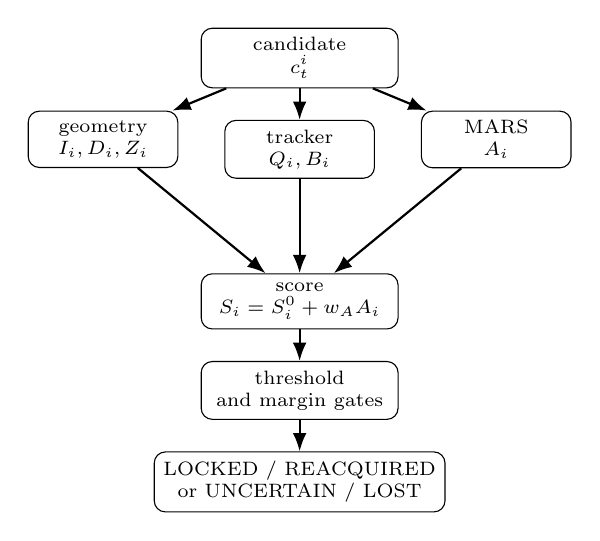
\begin{tikzpicture}[
    node distance=4mm,
    block/.style={draw, rounded corners, align=center, minimum width=25mm, minimum height=7mm, font=\scriptsize},
    small/.style={draw, rounded corners, align=center, minimum width=19mm, minimum height=6mm, font=\scriptsize},
    arrow/.style={-Latex, thick}
]
\node[block] (cand) {candidate\\$c_t^i$};
\node[small, below left=of cand] (geom) {geometry\\$I_i,D_i,Z_i$};
\node[small, below=of cand] (conf) {tracker\\$Q_i,B_i$};
\node[small, below right=of cand] (app) {MARS\\$A_i$};

\node[block, below=12mm of conf] (score) {score\\$S_i=S_i^0+w_AA_i$};
\node[block, below=of score] (accept) {threshold\\and margin gates};
\node[block, below=of accept] (state) {LOCKED / REACQUIRED\\or UNCERTAIN / LOST};

\draw[arrow] (cand) -- (geom);
\draw[arrow] (cand) -- (conf);
\draw[arrow] (cand) -- (app);
\draw[arrow] (geom) -- (score);
\draw[arrow] (conf) -- (score);
\draw[arrow] (app) -- (score);
\draw[arrow] (score) -- (accept);
\draw[arrow] (accept) -- (state);
\end{tikzpicture}
\caption{TIM-MARS candidate scoring and rejection flow. Geometry and tracker continuity define the base score, while MARS appearance is added only when available and gated.}
\label{fig:scoring_block}
\end{figure}


\subsection{Acceptance Threshold}

Let $c_t^\star$ be the highest-scoring candidate under $S_i$. The acceptance threshold depends on the previous memory state:
\begin{equation}
\tau_s =
\begin{cases}
\tau_L, & s_{t-1} = \mathrm{LOST},\\
\tau_K, & \mathrm{otherwise},
\end{cases}
\end{equation}
with
\begin{equation}
\tau_K = 0.52,
\quad
\tau_L = 0.60.
\end{equation}

If the candidate keeps the same tracker identity as the memory, the threshold is relaxed:
\begin{equation}
\tau_s' =
\max(0,\tau_s - \delta_{id}),
\quad
\delta_{id}=0.08.
\end{equation}

A candidate is rejected before acceptance if
\begin{equation}
S_t^\star < \tau_s'.
\end{equation}

\subsection{Conservative Appearance Rejection}

After a candidate passes the score threshold, TIM-MARS can still reject it using conservative appearance filtering.

Let $A^\star$ be the selected candidate raw appearance similarity, and let $A^{(2)}$ be the second-highest raw appearance similarity among candidates for which appearance was used and geometry allowed appearance. The appearance margin is
\begin{equation}
\Delta_A = A^\star - A^{(2)}.
\end{equation}

With conservative filtering enabled, the selected candidate is rejected if
\begin{equation}
A^\star < \tau_C
\lor
\Delta_A < \tau_M.
\end{equation}

For the hard re-entry evaluation,
\begin{equation}
\tau_C = 0.65,
\quad
\tau_M = 0.25.
\end{equation}

If appearance was not used, the missing-appearance rejection is
\begin{equation}
R_\emptyset =
\neg \mathrm{appearance\_used}(c_t^\star)
\land
\rho_A,
\end{equation}
where
\begin{equation}
\rho_A =
\begin{cases}
1, & \texttt{appearance\_conservative\_require\_appearance=true},\\
0, & \texttt{appearance\_conservative\_require\_appearance=false}.
\end{cases}
\end{equation}

The evaluated policy uses
\begin{equation}
\rho_A = 0.
\end{equation}
Therefore, missing appearance alone does not force a LOST state.

\subsection{State and Output}

The memory state is updated as
\begin{equation}
s_t =
\begin{cases}
\mathrm{REACQUIRED}, & s_{t-1}\in\{\mathrm{LOST},\mathrm{UNCERTAIN}\} \land \mathrm{accepted},\\
\mathrm{LOCKED}, & \mathrm{accepted},\\
\mathrm{UNCERTAIN}, & \mathrm{temporarily\ rejected},\\
\mathrm{LOST}, & \mathrm{rejected\ for\ too\ long}.
\end{cases}
\end{equation}

The control-facing output is
\begin{equation}
y_t =
\begin{cases}
b_t^\star, & s_t\in\{\mathrm{LOCKED},\mathrm{REACQUIRED}\},\\
\emptyset, & s_t\in\{\mathrm{UNCERTAIN},\mathrm{LOST},\mathrm{NO\_TARGET}\}.
\end{cases}
\end{equation}

This implements the control-safety rule: ambiguous identity evidence should produce no target rather than an unsafe wrong target.

\section{TIM-MARS Algorithm}

Algorithm~\ref{alg:tim_mars} summarises the implementation-level update used by TIM-MARS.

\begin{algorithm}[t]
\caption{TIM-MARS selected-target memory update}
\label{alg:tim_mars}
\begin{algorithmic}[1]
\REQUIRE tracker candidates $\mathcal{C}_t$, previous memory $m_{t-1}$
\ENSURE output target $y_t$, state $s_t$
\STATE discard candidates with $q_t^i < \tau_q$
\IF{$\mathcal{C}_t' = \emptyset$}
    \STATE update missing-frame counter
    \STATE $s_t \leftarrow \mathrm{UNCERTAIN}$ or $\mathrm{LOST}$
    \STATE $y_t \leftarrow \emptyset$
    \RETURN
\ENDIF
\FORALL{$c_t^i \in \mathcal{C}_t'$}
    \STATE compute $I_i$, $D_i$, $Z_i$, $Q_i$, and $B_i$
    \STATE compute base score $S_i^0$
\ENDFOR
\STATE compute base ambiguity margin $\Delta_t^0$
\STATE decide whether appearance should be used
\FORALL{$c_t^i \in \mathcal{C}_t'$}
    \IF{appearance is available and geometry allows appearance}
        \STATE compute raw MARS similarity $A_i$
        \IF{appearance is enabled and $A_i \geq \tau_A$}
            \STATE $S_i \leftarrow \mathrm{clip}(S_i^0+w_AA_i,0,1)$
        \ELSE
            \STATE $S_i \leftarrow S_i^0$
        \ENDIF
    \ELSE
        \STATE $S_i \leftarrow S_i^0$
    \ENDIF
\ENDFOR
\STATE $c_t^\star \leftarrow \arg\max_{c_t^i \in \mathcal{C}_t'} S_i$
\STATE choose threshold $\tau_s$ from previous state
\IF{$id(c_t^\star) = id_{t-1}^\star$}
    \STATE relax threshold by $\delta_{id}$
\ENDIF
\IF{$S_t^\star < \tau_s$}
    \STATE $s_t \leftarrow \mathrm{UNCERTAIN}$ or $\mathrm{LOST}$
    \STATE $y_t \leftarrow \emptyset$
    \RETURN
\ENDIF
\IF{conservative appearance filtering is enabled}
    \IF{appearance was not used and appearance is required}
        \STATE $s_t \leftarrow \mathrm{UNCERTAIN}$ or $\mathrm{LOST}$
        \STATE $y_t \leftarrow \emptyset$
        \RETURN
    \ENDIF
    \IF{appearance was used and $(A^\star < \tau_C$ or $\Delta_A < \tau_M)$}
        \STATE $s_t \leftarrow \mathrm{UNCERTAIN}$ or $\mathrm{LOST}$
        \STATE $y_t \leftarrow \emptyset$
        \RETURN
    \ENDIF
\ENDIF
\IF{previous state was $\mathrm{UNCERTAIN}$ or $\mathrm{LOST}$}
    \STATE $s_t \leftarrow \mathrm{REACQUIRED}$
\ELSE
    \STATE $s_t \leftarrow \mathrm{LOCKED}$
\ENDIF
\STATE update selected-target memory
\STATE update appearance memory only in confirmed LOCKED state
\STATE $y_t \leftarrow b_t^\star$
\end{algorithmic}
\end{algorithm}

Figure~\ref{fig:state_machine} shows the state-machine interpretation.

\begin{figure}[t]
\centering
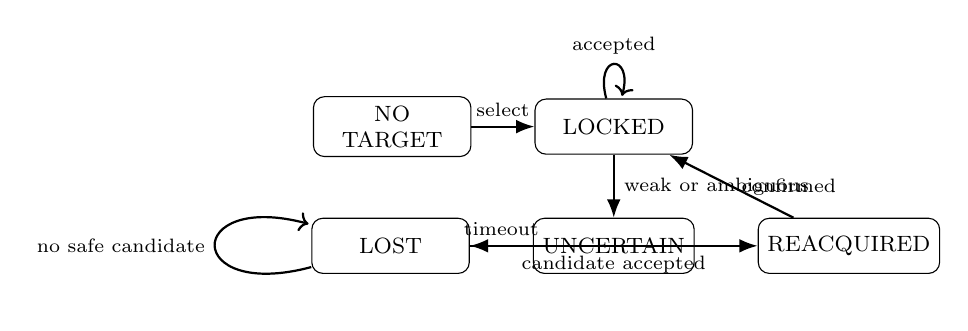
\begin{tikzpicture}[
    node distance=8mm,
    state/.style={draw, rounded corners, align=center, minimum width=20mm, minimum height=7mm, font=\footnotesize},
    arrow/.style={-Latex, thick, font=\scriptsize}
]
\node[state] (no) {NO\\TARGET};
\node[state, right=of no] (locked) {LOCKED};
\node[state, below=of locked] (uncertain) {UNCERTAIN};
\node[state, left=of uncertain] (lost) {LOST};
\node[state, right=of uncertain] (reacq) {REACQUIRED};

\draw[arrow] (no) -- node[above] {select} (locked);
\draw[arrow] (locked) -- node[right] {weak or ambiguous} (uncertain);
\draw[arrow] (uncertain) -- node[above] {timeout} (lost);
\draw[arrow] (lost) -- node[below] {candidate accepted} (reacq);
\draw[arrow] (reacq) -- node[right] {confirmed} (locked);
\draw[arrow] (locked) edge[loop above] node {accepted} (locked);
\draw[arrow] (lost) edge[loop left] node {no safe candidate} (lost);
\end{tikzpicture}
\caption{TIM-MARS state-machine interpretation. Ambiguous candidates are rejected into UNCERTAIN or LOST instead of being published as control-valid targets.}
\label{fig:state_machine}
\end{figure}

\section{Experimental Setup}

\subsection{Scenario}

The main evaluation uses a hard re-entry sequence with two people. The selected target is the black-shirt person. The sequence includes crossing, occlusion, identity ambiguity, and re-entry. These conditions stress the ability of the system to preserve the selected target rather than simply maintain any person track.

\subsection{Compared Trackers}

Three base tracker settings are evaluated:

\begin{itemize}
    \item ByteTrack;
    \item OCSORT;
    \item DeepSORT-MARS.
\end{itemize}

For each tracker, the raw selected target is compared against the TIM-MARS selected-target output when available.

\subsection{Metrics}

The evaluation separates selected-target output into three main categories:

\begin{itemize}
    \item correct: the output corresponds to the true selected person;
    \item wrong: the output corresponds to another person;
    \item lost: no valid selected-target output is available while the selected person is visible.
\end{itemize}

The primary ratios are computed over the visible target duration:

\begin{equation}
r_\mathrm{correct} = \frac{t_\mathrm{correct}}{t_\mathrm{visible}},
\end{equation}

\begin{equation}
r_\mathrm{wrong} = \frac{t_\mathrm{wrong}}{t_\mathrm{visible}},
\end{equation}

\begin{equation}
r_\mathrm{lost} = \frac{t_\mathrm{lost}}{t_\mathrm{visible}}.
\end{equation}

The most important safety metric is wrong-target duration.

\subsection{Runtime Measurement Scope}

The runtime comparison isolates the post-detection tracking and selected-target memory stack. The source bag replays \texttt{/camera/image\_raw} and \texttt{/detections}, while Hailo inference is excluded. This makes the comparison suitable for measuring tracker and TIM-MARS overhead under identical detector outputs, but it should not be interpreted as full onboard perception-pipeline runtime.

\section{Results}

Table~\ref{tab:hard_reentry_results} reports selected-target correctness as percentages of the visible-target interval. Figure~\ref{fig:result_ratios} visualises the same comparison, and Figure~\ref{fig:qualitative_hard_reentry} shows a qualitative hard re-entry example.

\begin{table}[t]
\centering
\caption{Selected-target correctness on the hard re-entry sequence. Values are percentages of the visible-target interval.}
\label{tab:hard_reentry_results}
\begin{tabular}{llccc}
\toprule
Tracker & Variant & Correct & Wrong & Lost \\
\midrule
ByteTrack & Raw & 68.7 & 11.5 & 19.8 \\
ByteTrack & TIM-MARS & \textbf{96.9} & 1.5 & \textbf{1.6} \\
DeepSORT-MARS & Raw & 92.8 & \textbf{0.0} & 7.2 \\
DeepSORT-MARS & TIM-MARS & 92.3 & 5.1 & 2.6 \\
OCSORT & Raw & 48.7 & 35.6 & 15.7 \\
OCSORT & TIM-MARS & 67.2 & 11.9 & 20.9 \\
\bottomrule
\end{tabular}
\end{table}

\begin{figure}[t]
\centering
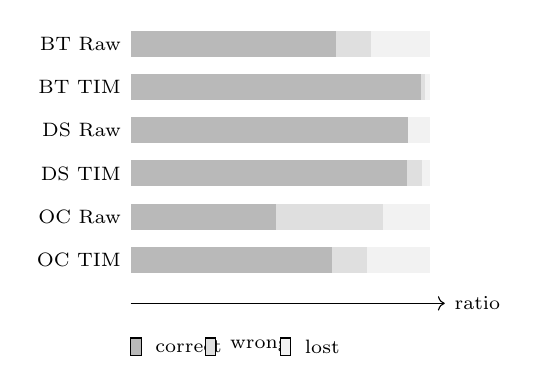
\begin{tikzpicture}[
    x=38mm,
    y=5.5mm,
    font=\scriptsize
]
\draw[->] (0,0) -- (1.05,0) node[right] {ratio};

\node[anchor=east] at (0,6) {BT Raw};
\fill[gray!55] (0,5.7) rectangle (0.687,6.3);
\fill[gray!25] (0.687,5.7) rectangle (0.802,6.3);
\fill[gray!10] (0.802,5.7) rectangle (1.000,6.3);

\node[anchor=east] at (0,5) {BT TIM};
\fill[gray!55] (0,4.7) rectangle (0.969,5.3);
\fill[gray!25] (0.969,4.7) rectangle (0.984,5.3);
\fill[gray!10] (0.984,4.7) rectangle (1.000,5.3);

\node[anchor=east] at (0,4) {DS Raw};
\fill[gray!55] (0,3.7) rectangle (0.928,4.3);
\fill[gray!25] (0.928,3.7) rectangle (0.928,4.3);
\fill[gray!10] (0.928,3.7) rectangle (1.000,4.3);

\node[anchor=east] at (0,3) {DS TIM};
\fill[gray!55] (0,2.7) rectangle (0.923,3.3);
\fill[gray!25] (0.923,2.7) rectangle (0.974,3.3);
\fill[gray!10] (0.974,2.7) rectangle (1.000,3.3);

\node[anchor=east] at (0,2) {OC Raw};
\fill[gray!55] (0,1.7) rectangle (0.487,2.3);
\fill[gray!25] (0.487,1.7) rectangle (0.843,2.3);
\fill[gray!10] (0.843,1.7) rectangle (1.000,2.3);

\node[anchor=east] at (0,1) {OC TIM};
\fill[gray!55] (0,0.7) rectangle (0.672,1.3);
\fill[gray!25] (0.672,0.7) rectangle (0.791,1.3);
\fill[gray!10] (0.791,0.7) rectangle (1.000,1.3);

\node[anchor=west] at (0.05,-1.0) {correct};
\draw[fill=gray!55] (0,-1.2) rectangle (0.035,-0.8);
\node[anchor=west] at (0.30,-1.0) {wrong};
\draw[fill=gray!25] (0.25,-1.2) rectangle (0.285,-0.8);
\node[anchor=west] at (0.55,-1.0) {lost};
\draw[fill=gray!10] (0.50,-1.2) rectangle (0.535,-0.8);
\end{tikzpicture}
\caption{Stacked selected-target correctness ratios. TIM-MARS strongly reduces wrong-target output for ByteTrack and OCSORT.}
\label{fig:result_ratios}
\end{figure}

\begin{figure*}[t]
\centering
\begin{tabular}{cccc}
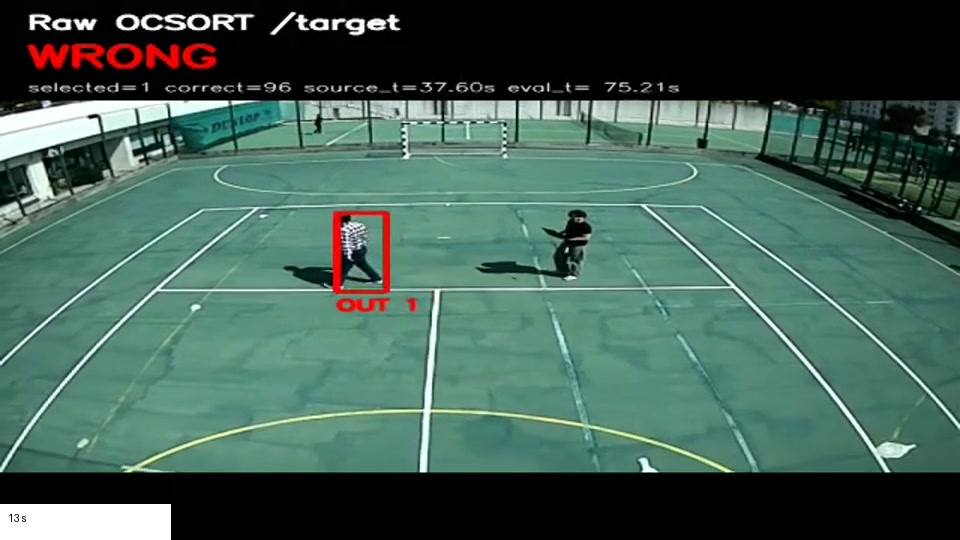
\includegraphics[width=0.235\textwidth]{figures/qual_raw_wrong_crop.jpg} &
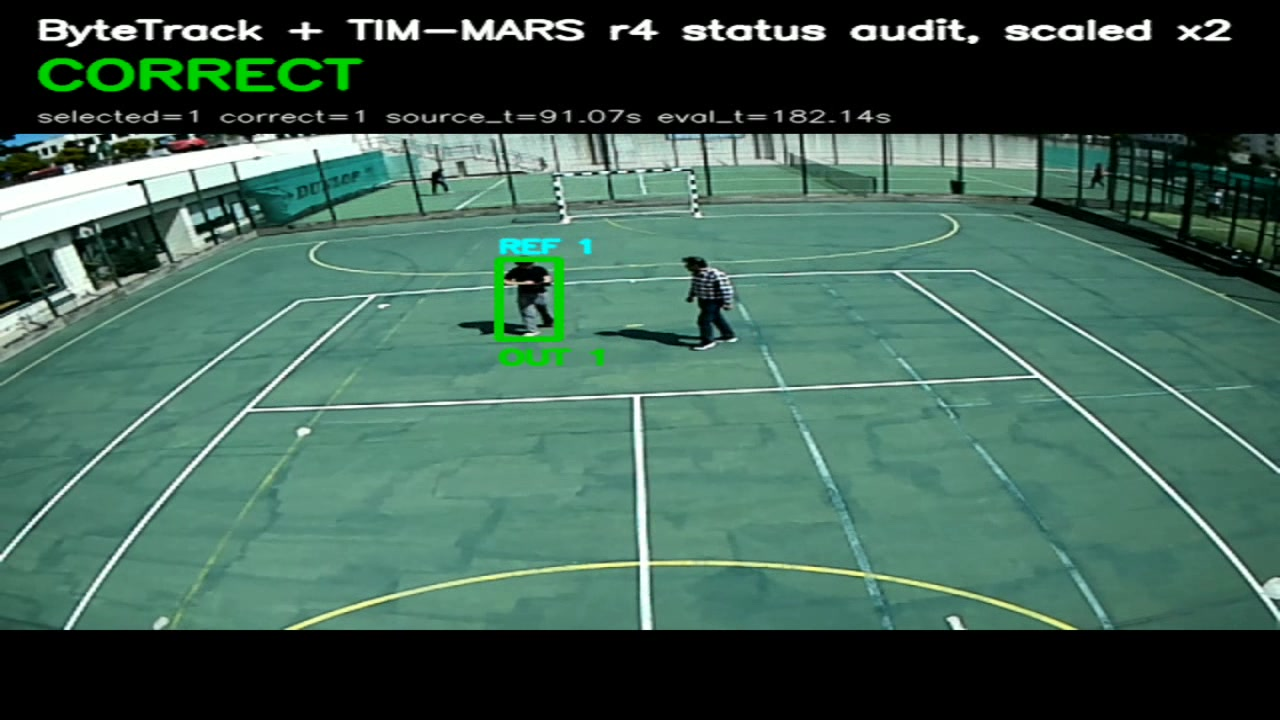
\includegraphics[width=0.235\textwidth]{figures/qual_tim_safe.jpg} &
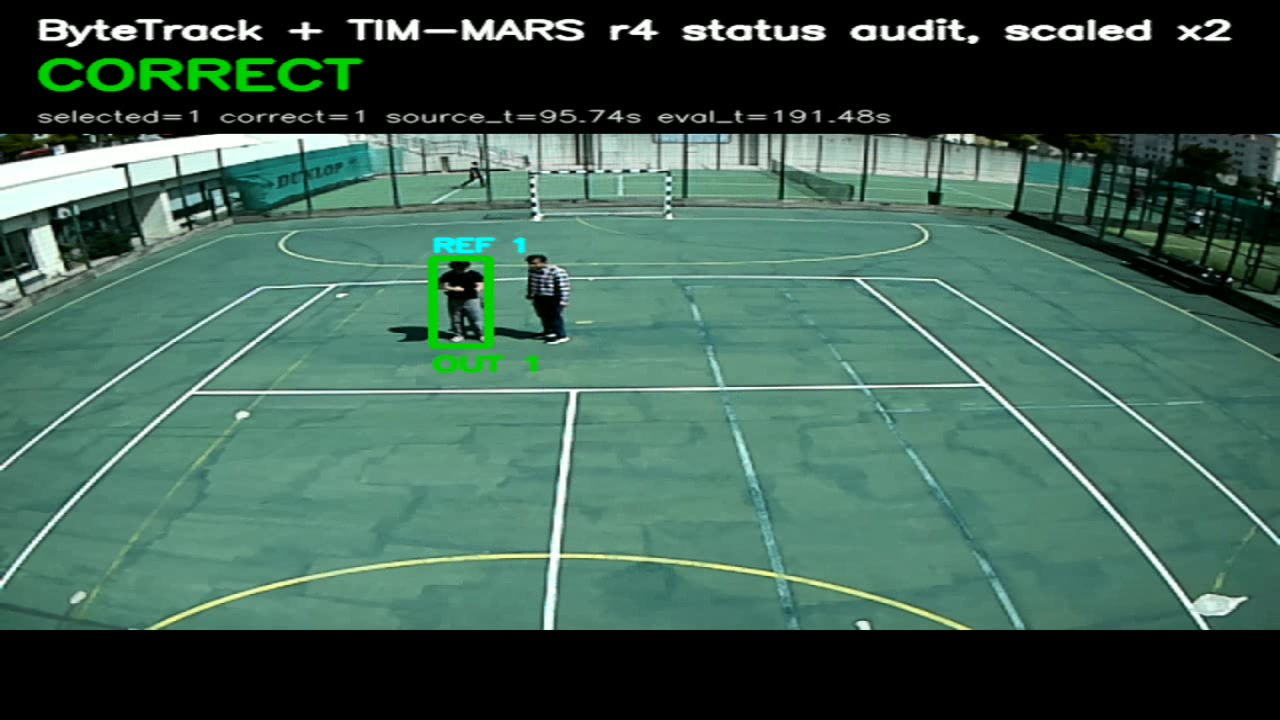
\includegraphics[width=0.235\textwidth]{figures/qual_reentry.jpg} &
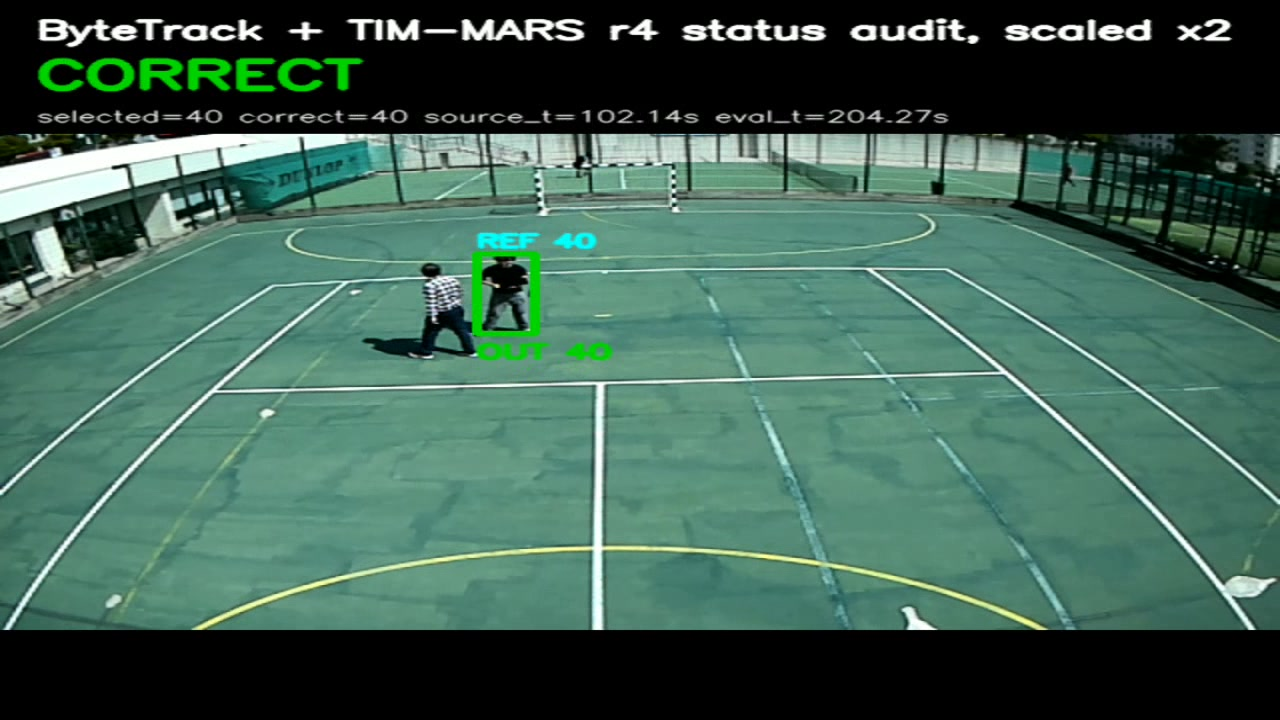
\includegraphics[width=0.235\textwidth]{figures/qual_reacquired.jpg} \\
(a) Raw OCSORT error &
(b) TIM-MARS correct selection &
(c) Close re-entry ambiguity &
(d) Correct identity recovery
\end{tabular}
\caption{Qualitative examples from the hard re-entry sequence. Panel (a) shows a representative raw selected-target failure, where the output persists on the wrong person. Panels (b)--(d) show ByteTrack + TIM-MARS maintaining and recovering the intended target identity after close interaction, even when the numeric tracker ID changes.}
\label{fig:qualitative_hard_reentry}
\end{figure*}


ByteTrack benefits most from TIM-MARS. Correct selected-target output increases from 68.7\% to 96.9\%, while wrong-target output decreases from 11.5\% to 1.5\%. Lost-target output also decreases from 19.8\% to 1.6\%. This indicates that the base tracker had recoverable identity instability and that TIM-MARS improved both safety and continuity.

DeepSORT-MARS is already a strong raw baseline, with 92.8\% correct output and 0.0\% wrong output. Adding TIM-MARS reduces lost output from 7.2\% to 2.6\%, but introduces 5.1\% wrong output. Under the adopted safety rule, this is not a strict improvement.

OCSORT also benefits from TIM-MARS in terms of safety. Wrong-target output decreases from 35.6\% to 11.9\%, while correct output increases from 48.7\% to 67.2\%. Lost output increases from 15.7\% to 20.9\%. This is a valid safety trade-off, but remains weaker than the ByteTrack TIM-MARS result.

\subsection{Post-Detection Runtime}

Table~\ref{tab:final_compute_runtime} reports the final replay-level runtime comparison. This benchmark isolates the post-detection ROS stack: the same recorded \texttt{/detections} topic is replayed for each method, and Hailo inference is not included.

\begin{table*}[t]
\centering
\caption{Post-detection replay runtime for the final methods. Hailo inference is excluded; the same recorded detections are replayed for each method.}
\label{tab:final_compute_runtime}
\begin{tabular}{lrrrrrrr}
\toprule
Method & Output & Tracks & CPU & User CPU & Sys. CPU & Wall & Peak RSS \\
 & samples & samples & (\%) & (s) & (s) & time & (MB) \\
\midrule
Raw ByteTrack & 949 & 948 & 6 & 13.74 & 5.57 & 5:07.90 & 585.5 \\
ByteTrack $+$ TIM-MARS & 952 & 952 & 10 & 23.55 & 7.63 & 5:08.80 & 584.7 \\
Raw DeepSORT-MARS & 952 & 951 & 8 & 18.38 & 6.51 & 5:08.52 & 585.7 \\
Raw OCSORT & 953 & 952 & 7 & 17.33 & 5.84 & 5:07.89 & 585.6 \\
OCSORT $+$ TIM-MARS & 950 & 950 & 9 & 21.11 & 7.73 & 5:11.11 & 586.0 \\
\bottomrule
\end{tabular}
\end{table*}


ByteTrack + TIM-MARS increases replay-level CPU share from 6\% to 10\% relative to raw ByteTrack, while wall time and peak memory remain nearly unchanged. Compared with raw DeepSORT-MARS, ByteTrack + TIM-MARS uses slightly more CPU in this replay setup, but achieves the strongest selected-target correctness on the evaluated hard re-entry sequence. The appropriate conclusion is therefore not that TIM-MARS is cheaper than DeepSORT-MARS, but that it provides the best robustness result with modest post-detection overhead.

\section{Discussion}

The results support a narrow but important claim: selected-target memory can improve control-facing target robustness when the base tracker has recoverable identity instability. This is clearest for ByteTrack, where TIM-MARS increases correct selected-target output and reduces both wrong and lost output on the hard re-entry sequence.

The DeepSORT-MARS result is a useful counterexample. Raw DeepSORT-MARS already produces 0.0\% wrong-target output on this sequence. Adding TIM-MARS reduces lost output, but introduces wrong-target output. Under the adopted safety rule, this is not a strict improvement. This prevents the paper from claiming that TIM-MARS is universally beneficial across all trackers.

The OCSORT result shows a different trade-off. TIM-MARS reduces wrong-target output substantially, from 35.6\% to 11.9\%, but increases lost output from 15.7\% to 20.9\%. This is acceptable only under the control-safety assumption that LOST is safer than following the wrong person.

The main limitation is evaluation scope. The current evidence is based on a hard re-entry stress sequence, not a broad dataset-level benchmark. The result should therefore be interpreted as a focused validation of the selected-target memory mechanism rather than a general claim about all UAV person-following scenarios.

A second limitation is tracker dependence. TIM-MARS relies on the base tracker producing usable candidate tracks. If the tracker is too fragmented, memory can either become overly conservative or select a wrong candidate. The method is therefore best understood as a control-safety layer above a tracker, not as a replacement for robust multi-object tracking.

\subsection{Why Not Use DeepSORT-MARS Alone?}

The DeepSORT-MARS baseline is intentionally included because it is a strong appearance-based tracker. On the evaluated hard re-entry sequence, raw DeepSORT-MARS achieves 0.0\% wrong-target output, which makes it a strong safety baseline. TIM-MARS should therefore not be interpreted as a universal replacement for appearance-based tracking.

The distinction is instead architectural. DeepSORT-MARS addresses general multi-object association: it decides which detections belong to which tracks. TIM-MARS addresses the downstream selected-target control question: whether a candidate track should currently be published as the selected target, rejected as unsafe, or recovered after re-entry. This distinction matters for UAV following because a temporary lost-target state can be handled conservatively, while a wrong selected target may drive the vehicle toward the wrong person.

The results support this narrower interpretation. TIM-MARS is most useful when the base tracker has recoverable selected-identity instability, as shown by the ByteTrack result. When the base tracker is already stable under the selected-target safety metric, as in raw DeepSORT-MARS on this sequence, adding TIM-MARS can be unnecessary or even harmful. The contribution is therefore not a new generic MOT tracker, but a tracker-agnostic selected-target memory layer and evaluation protocol for control-facing person following.


\section{Conclusion}

This paper presented TIM-MARS, a selected-target memory layer for vision-based UAV person following. Rather than replacing the multi-object tracker, TIM-MARS operates above it and publishes a control-facing target state using geometric continuity, tracker state, and MARS appearance evidence.

On the evaluated hard re-entry sequence, ByteTrack + TIM-MARS provided the strongest selected-target result, increasing correct-target output from 68.7\% to 96.9\% and reducing wrong-target output from 11.5\% to 1.5\%. The replay-level runtime results show that this improvement comes with modest post-detection overhead: CPU share increased from 6\% to 10\% relative to raw ByteTrack, while wall time and peak memory remained nearly unchanged.

The results also show that TIM-MARS is not universally beneficial. Raw DeepSORT-MARS already achieved 0.0\% wrong-target output on this sequence, and adding TIM-MARS introduced wrong-target output. This supports the main conclusion of the paper: selected-target memory is most useful when the base tracker has recoverable identity instability, and it must be evaluated with control-oriented correct, wrong, and lost output durations.

Future work will validate the method across more sequences and full onboard Hailo-based flight experiments, including closed-loop behaviours that treat wrong-target output as less safe than temporary target loss.


\bibliographystyle{IEEEtran}
\bibliography{references}

\end{document}
